%% For double-blind review submission, w/o CCS and ACM Reference (max submission space)
\documentclass[sigplan,review,anonymous]{acmart}\settopmatter{printfolios=true,printccs=false,printacmref=false}
%% For double-blind review submission, w/ CCS and ACM Reference
%\documentclass[sigplan,review,anonymous]{acmart}\settopmatter{printfolios=true}
%% For single-blind review submission, w/o CCS and ACM Reference (max submission space)
%\documentclass[sigplan,review]{acmart}\settopmatter{printfolios=true,printccs=false,printacmref=false}
%% For single-blind review submission, w/ CCS and ACM Reference
%\documentclass[sigplan,review]{acmart}\settopmatter{printfolios=true}
%% For final camera-ready submission, w/ required CCS and ACM Reference
%\documentclass[sigplan]{acmart}\settopmatter{}


%% Conference information
%% Supplied to authors by publisher for camera-ready submission;
%% use defaults for review submission.
\acmConference[PL'18]{ACM SIGPLAN Conference on Programming Languages}{January 01--03, 2018}{New York, NY, USA}
\acmYear{2018}
\acmISBN{} % \acmISBN{978-x-xxxx-xxxx-x/YY/MM}
\acmDOI{} % \acmDOI{10.1145/nnnnnnn.nnnnnnn}
\startPage{1}

%% Copyright information
%% Supplied to authors (based on authors' rights management selection;
%% see authors.acm.org) by publisher for camera-ready submission;
%% use 'none' for review submission.
\setcopyright{none}
%\setcopyright{acmcopyright}
%\setcopyright{acmlicensed}
%\setcopyright{rightsretained}
%\copyrightyear{2018}           %% If different from \acmYear

%% Bibliography style
\bibliographystyle{ACM-Reference-Format}
%% Citation style
%\citestyle{acmauthoryear}  %% For author/year citations
%\citestyle{acmnumeric}     %% For numeric citations
%\setcitestyle{nosort}      %% With 'acmnumeric', to disable automatic
                            %% sorting of references within a single citation;
                            %% e.g., \cite{Smith99,Carpenter05,Baker12}
                            %% rendered as [14,5,2] rather than [2,5,14].
%\setcitesyle{nocompress}   %% With 'acmnumeric', to disable automatic
                            %% compression of sequential references within a
                            %% single citation;
                            %% e.g., \cite{Baker12,Baker14,Baker16}
                            %% rendered as [2,3,4] rather than [2-4].


%%%%%%%%%%%%%%%%%%%%%%%%%%%%%%%%%%%%%%%%%%%%%%%%%%%%%%%%%%%%%%%%%%%%%%
%% Note: Authors migrating a paper from traditional SIGPLAN
%% proceedings format to PACMPL format must update the
%% '\documentclass' and topmatter commands above; see
%% 'acmart-pacmpl-template.tex'.
%%%%%%%%%%%%%%%%%%%%%%%%%%%%%%%%%%%%%%%%%%%%%%%%%%%%%%%%%%%%%%%%%%%%%%


%% Some recommended packages.
\usepackage{booktabs}   %% For formal tables:
                        %% http://ctan.org/pkg/booktabs
\usepackage{subcaption} %% For complex figures with subfigures/subcaptions
                        %% http://ctan.org/pkg/subcaption
\usepackage{algorithm}
\usepackage{color}
\newcommand\mingcan[1]{\noindent{\color{green} {\bf \fbox{mingcan}} {\it#1}}}
%\renewcommand{\algorithmcfname}{ALGORITHM}
\usepackage[noend]{algorithmic}

\begin{document}

%% Title information
\title[Short Title]{Decentralized Multi-Factor Based Scheduling Framework for Asymmetric Multicore Processors}         %% [Short Title] is optional;
                                        %% when present, will be used in
                                        %% header instead of Full Title.
%\titlenote{with title note}             %% \titlenote is optional;
                                        %% can be repeated if necessary;
                                        %% contents suppressed with 'anonymous'
%\subtitle{Subtitle}                     %% \subtitle is optional
%\subtitlenote{with subtitle note}       %% \subtitlenote is optional;
                                        %% can be repeated if necessary;
                                        %% contents suppressed with 'anonymous'


%% Author information
%% Contents and number of authors suppressed with 'anonymous'.
%% Each author should be introduced by \author, followed by
%% \authornote (optional), \orcid (optional), \affiliation, and
%% \email.
%% An author may have multiple affiliations and/or emails; repeat the
%% appropriate command.
%% Many elements are not rendered, but should be provided for metadata
%% extraction tools.

%% Author with single affiliation.
\author{First1 Last1}
\authornote{with author1 note}          %% \authornote is optional;
                                        %% can be repeated if necessary
\orcid{nnnn-nnnn-nnnn-nnnn}             %% \orcid is optional
\affiliation{
  \position{Position1}
  \department{Department1}              %% \department is recommended
  \institution{Institution1}            %% \institution is required
  \streetaddress{Street1 Address1}
  \city{City1}
  \state{State1}
  \postcode{Post-Code1}
  \country{Country1}                    %% \country is recommended
}
\email{first1.last1@inst1.edu}          %% \email is recommended

%% Author with two affiliations and emails.
\author{First2 Last2}
\authornote{with author2 note}          %% \authornote is optional;
                                        %% can be repeated if necessary
\orcid{nnnn-nnnn-nnnn-nnnn}             %% \orcid is optional
\affiliation{
  \position{Position2a}
  \department{Department2a}             %% \department is recommended
  \institution{Institution2a}           %% \institution is required
  \streetaddress{Street2a Address2a}
  \city{City2a}
  \state{State2a}
  \postcode{Post-Code2a}
  \country{Country2a}                   %% \country is recommended
}
\email{first2.last2@inst2a.com}         %% \email is recommended
\affiliation{
  \position{Position2b}
  \department{Department2b}             %% \department is recommended
  \institution{Institution2b}           %% \institution is required
  \streetaddress{Street3b Address2b}
  \city{City2b}
  \state{State2b}
  \postcode{Post-Code2b}
  \country{Country2b}                   %% \country is recommended
}
\email{first2.last2@inst2b.org}         %% \email is recommended
%\usepackage{color}
%\newcommand\mingcan[1]{\noindent{\color{green} {\bf \fbox{mingcan}} {\it#1}}}

%% Abstract
%% Note: \begin{abstract}...\end{abstract} environment must come
%% before \maketitle command
\begin{abstract}
Asymmetric multicore processors (AMP) are necessary for extracting performance in an era of limited power budget and dark silicon. Despite becoming increasingly prevalent, our software fails to use them efficiently. OS schedulers, in particular, handle asymmetry only under restricted scenarios, if at all. We have efficient symmetric schedulers, efficient asymmetric schedulers for single-threaded workloads, and efficient asymmetric schedulers for single program workloads. What we do not have is a scheduler that can handle all three factors affecting AMP scheduling: core affinity, thread criticality, and scheduling fairness.

To address this problem, this paper introduces the first general purpose asymmetry-aware scheduler targeting multi-threaded multi-programmed workloads. It estimates the performance of each thread on each type of core and it identifies communication patterns and bottleneck threads. With this information, the scheduler makes coordinated core assignment and thread selection decisions that still provide each application its fair share of the processor's time.

 We evaluated our approach on GEM5 through four distinct big.LITTLE configurations and 26 multi-threaded multi-programmed workloads composed of PARSEC and SPLASH2 benchmarks. Compared against the Linux CFS scheduler and a state-of-the-art AMP-aware scheduler, we demonstrate performance gains of up to 25\% and 5\% to 15\% on average depending on the hardware setup.
\end{abstract}


%% 2012 ACM Computing Classification System (CSS) concepts
%% Generate at 'http://dl.acm.org/ccs/ccs.cfm'.
\begin{CCSXML}
<ccs2012>
<concept>
<concept_id>10011007.10011006.10011008</concept_id>
<concept_desc>Software and its engineering~General programming languages</concept_desc>
<concept_significance>500</concept_significance>
</concept>
<concept>
<concept_id>10003456.10003457.10003521.10003525</concept_id>
<concept_desc>Social and professional topics~History of programming languages</concept_desc>
<concept_significance>300</concept_significance>
</concept>
</ccs2012>
\end{CCSXML}

\ccsdesc[500]{Software and its engineering~General programming languages}
\ccsdesc[300]{Social and professional topics~History of programming languages}
%% End of generated code


%% Keywords
%% comma separated list
\keywords{runtime, scheduler, asymmetric multicore processor}  %% \keywords are mandatory in final camera-ready submission


%% \maketitle
%% Note: \maketitle command must come after title commands, author
%% commands, abstract environment, Computing Classification System
%% environment and commands, and keywords command.
\maketitle

\section{Introduction}
\label{itr}
For decades, heterogeneous multicore processors have been verified to be a trend for both academia and industry against homogeneous multicore processors. More specific, single-ISA asymmetric multicore processor (AMP) provides a new opportunity to further improve system performance with low energy consumption than traditional symmetric multicore processors (SMP).  This advantage is fundamentally achieved by the heterogeneous hardware support in AMP: High-performance out-of-order big core to improve performance and low-energy in-order little core to save energy.  

Followed by the development of AMPs and multi-thread parallel programs, improving system performance by efficient OS scheduler with heterogeneous hardware support has become a main concern in the literature \cite{mittal2016survey}. Global scheduling framework \cite{jeff2013big} enables flexible selection of all possible threads for each core to achieve efficient resource share, while asymmetric hardware resources and multi-thread workloads make the scheduling space much more complex than before. To illustrate the challenges, we briefly present below three main runtime issues for scheduling multi-thread workloads on AMPs: fairness, bottleneck acceleration and core sensitivity:

%\begin{itemize}
%\item 
%\subsection*{Fairness}
\textbf{\textit{Fairness:}} To achieve high efficiency, a common requirement is to keep all resources busy with loads balanced and programs running in similar progress. Instead of running multiple single-thread applications in SMP, simple equal execution time cannot lead to equal progress in AMPs. 
%(3) similar loads in different type of cores doesn't means balancing.

\textbf{\textit{Bottleneck Acceleration:}} Bottleneck threads or code segments will block other threads due to data dependence, and thus critically influence the system throughput and program turnaround time. For multi-thread multiprogram co-execution on AMP, we need to handle multiple bottlenecks simultaneously.  
%(1) we can not easily identify how critical a thread is by measuring how much time other threads waiting it in total - the blocked time on heterogeneous cores are incomparable directly; (2) we cannot predict how long the critical code segment is and 
%there is a trade-off between executing it in current core right now or migrating it to a high performance core first for further acceleration.  
 %\item

\textbf{\textit{Core Sensitivity:}} Workloads and application threads have different sensitivities regarding heterogeneous hardware resources. Different from executing on SMPs, we want to execute threads on suited type of cores in AMPs. To achieve this efficiently, we need (1) to rank ready threads relatively based on their predicted speedup; (2) to map higher speedup threads to high-performance cores and enqueue correspondingly to avoid triggering additional further migration between cores when executing.
%\end{itemize}

Multiple efforts from research communities have been devoted to addressing those issues, such as \cite{han2018multicore,chronaki2017task,joao2012bottleneck,suleman2009accelerating,du2013criticality} for bottleneck and critical section acceleration, \cite{zahedi2018amdahl,wang2016rebudget,van2012scheduling,li2009efficient,li2007efficient} for fairness and \cite{cao2012yin,kumar2004single,becchi2006dynamic} for core sensitivity or multi-factor mixed model as \cite{kim2018exploring,kim2016fairness,saez2012leveraging,van2013fairness,joao2013utility,jibaja2016portable}. 
In brief, fairness-oriented approaches have demonstrated their efficiency on multiprogram co-executed workloads with single-thread applications as precise mathematical analysis can be constructed \cite{kim2016fairness, kim2018exploring}. Bottleneck acceleration methods equipped with a runtime core sensitivity model have shown significant advantage on multi-thread applications in general single-program workloads \cite{joao2012bottleneck,joao2013utility}. In addition, with more emphasis posed on fairness with help of VM one can also obtain a powerful multi-factor mixed model applied by the state-of-the-art AMP-aware scheduler \cite{jibaja2016portable}. 

To the best of knowledge, there are two problems remain in the VM-based multi-factor mixed model when it is targeting multi-thread multiprogram scheduling.   
%In brief, single-factor based approach can efficient deal with certain scenarios with limited workloads and runtime but losing generality. Multi-factor based approaches have been shown to be the trend to address general scheduling problem on AMPs with multi-thread workloads. 
%To the best of knowledge, there are two remain problems in the state-of-the-art multi-factor based approach:
\begin{itemize}
\item Mix-model loses information from original runtime and then makes no-precisely decisions with mixed priority. 
\item Guided by VM without direct kernel updating, thread selector can not collaborate with core allocator and both of them make local-optimal decisions.  
\end{itemize}
\begin{figure}
\centering
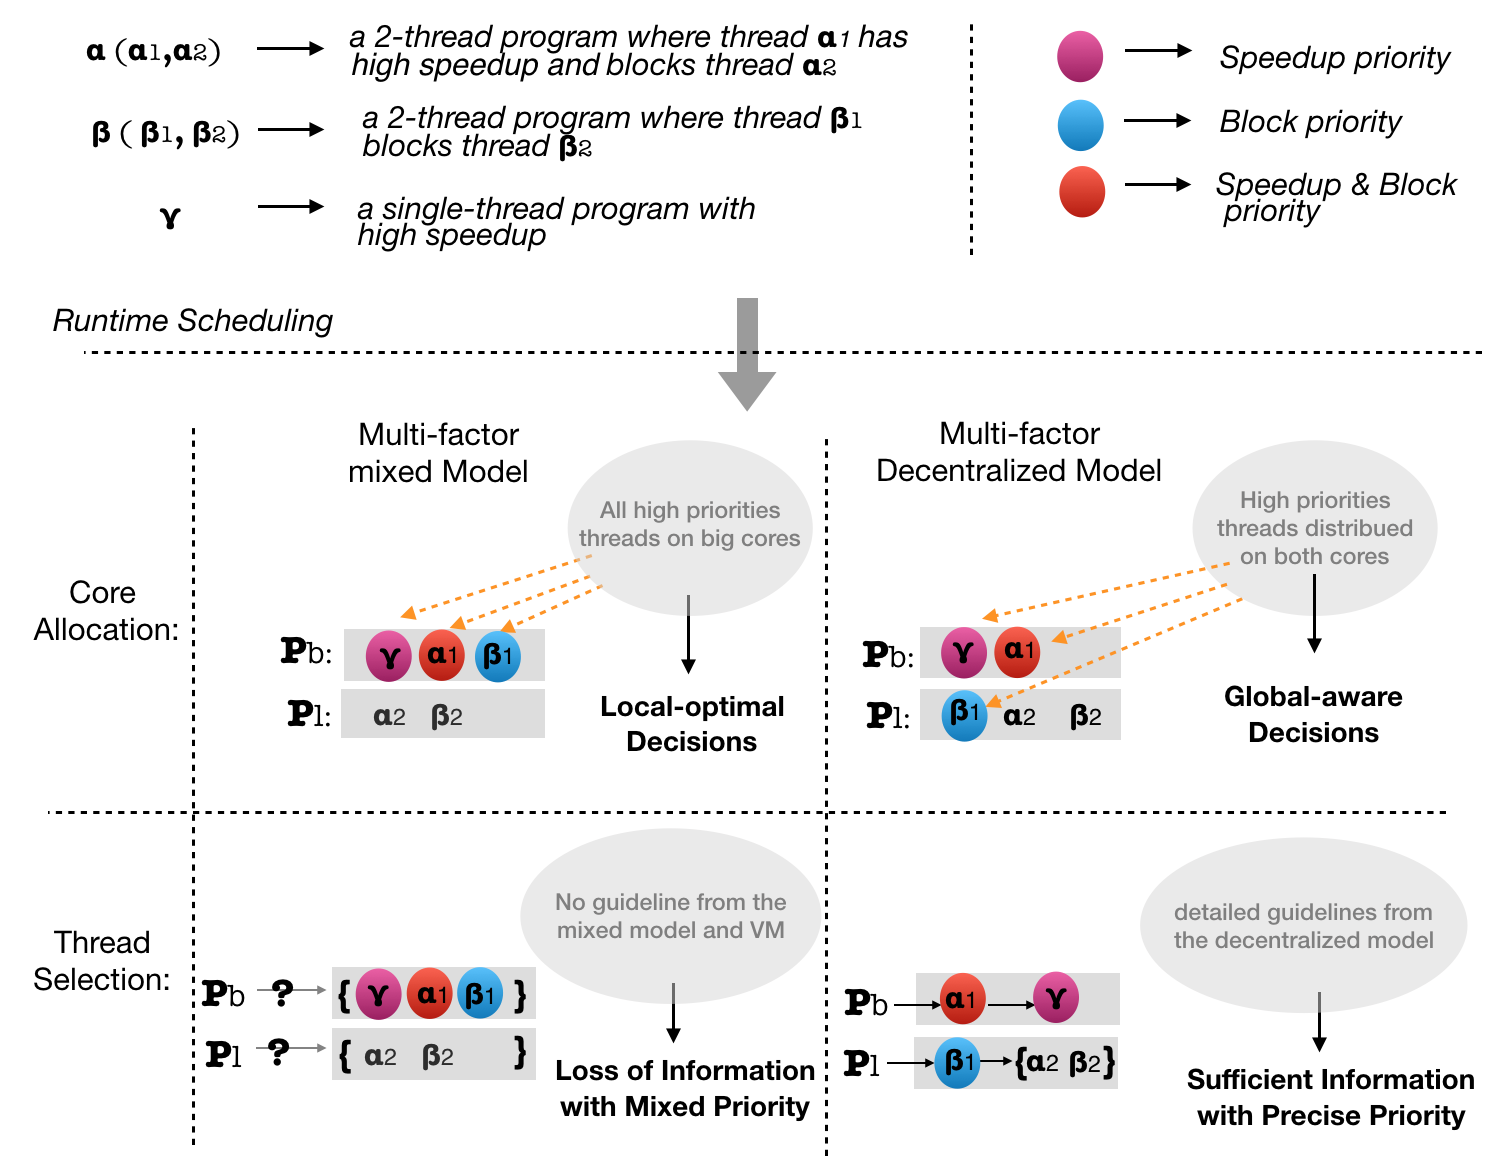
\includegraphics[scale=0.35]{figures/mt2.png}
\caption{Motivating Example: Multi-thread multiprogram co-executed workload on asymmetric multicore processors with a big core $P_b$ and a little core $P_l$}
\label{me}
\end{figure} 

To demonstrate the problems, consider a simple motivating example as shown in figure \ref{me} which we illustrate below:

\textbf{\textit{Motivating Example:}} Consider a simple AMP with a high-performance big core $P_b$ and a little core $P_l$. 
Let there be three co-executed applications: {$\alpha$, $\beta$, $\gamma$}. Both $\alpha$ and $\beta$ have two threads: $\alpha_1, \alpha_2, \beta_1, \beta_2$. The code segments of $\alpha_1, \beta_1$ block $\alpha_2, \beta_2$, separately. $\alpha_1$ has higher speedup on big core against $\beta_1$.  $\gamma$ is a single-thread application enjoying the highest speedup against other application threads. 
%There are a lot of parallel threads ready to be executed. We name the set of threads with high bottleneck level to be \{$t_b$\} and the set of threads with high predicted speedup to be \{$t_s$\}. 
Based on the multi-factor mixed model \cite{jibaja2016portable}, either the high speedup thread ($\gamma$) or blocking threads ($\alpha_1,\beta_1$) will have affinity on $P_b$ -{\it local-optimal decision}. When the thread selector on $P_b$ is invoked, no more guideline can be obtained from the thread affinity provided by the mixed model - {\it loss of information with mixed priority}. Instead, a better solution can be provided in a multi-factor decentralized model by only mapping the two high speedup threads ($\gamma,\alpha_1$) to $P_b$ and keeping the other blocking thread $\beta_1$ in $P_l$ - {\it global-aware decision}. Then the thread selector invoked by both $P_b$ and $P_l$ guided through the blocking priority, will select and accelerate bottleneck threads $\alpha_1,\beta_1$ locally and simultaneously without waiting each other - {\it sufficient information with precise priority}.  

%both of them will get high priority and be affiliated on the big core. Thus, some of those high priority threads need to be waited in the runqueue of $p_b$. Further, when $p_b$ is ready to select the next task, it may select a $t_s$ first instead of a $t_b$ as the original bottleneck priority has lost after setup its affinity. In brief, the core allocator made the first {\it selfish} greedy decision to enqueue those high priority threads on big core without leaving a better solution space for thread selector. Second, the thread selector lose original information and cannot guarantee to make a good decision. With efficient preemption mechanism, $p_l$ can select a $t_b$ even from $p_b$'s runqueue, but this leads to additional overhead from migration. If the core allocator and thread selector can be collaborated, a trivial better solution in this example can be $p_b$ running \{$t_s \cap t_b$\} whilst $p_l$ running \{$t_b$\}. 

%The first problem is obvious as in runtime scheduling, every change in a current decision will influence the future solution space and there is no way to predict it especially for asymmetric multicore processors with multiple multi-thread workloads.  
%To demonstrate the second problem, scheduling a ready thread from a run-queue in big core to be executed in a ready little core can result in an optimal solution from a greedy point of view, or we say a {\it current} optimal solution. But if this thread will only run on the little core for a tidy bit of time and then move back to a big core by preemption when the big core is ready, the overall runtime overhead from additional migrations may totally defeat the benefit from the hard and useless work on the little core. A high level motivating example is shown in Fig \ref{mt}, where $\mathcal{T}$ is a high priority thread which just ranked in the second position under the current running thread on big core's run-queue. By global scheduling, a ready little core will decide to run this high priority thread $\mathcal{T}$ and migrate it from big core's run-queue. While the problem happens if the big core finish its current thread right after the migration issued by the little core, as the big core will decide to run $\mathcal{T}$ and move it back by preemption. Those frequent runtime selections and migrations do lower the performance in this case.

So instead of optimizing the core allocation and thread selection functions one by one and dealing with multiple factors in a mixed central model, we come up with a collaboration-based runtime framework to address those problems. In brief, our proposed framework equipped with a multi-factor {\it decentralized} model - different runtime factors are distributed to be mainly addressed by different functional units of the scheduler, including core allocator, thread selector and preemption trigger. Decisions in each functional unit are directly guided by priorities from sufficient runtime without losing information through a mixed central model. Those decisions only aim to benefit each of their targeting factors and avoid making trouble for each other, so neither greedy nor local-optimal from a multi-factor point of view. Then all those sub-decisions from different functional units in scheduler dynamically collaborate together to result in overall smarter scheduling decisions during runtime. 

We summarise our main contributions:
\begin{itemize}
\item[1.] {\it A runtime multi-factor decentralized model targeting multi-thread multiprogram workloads provides new opportunities for further performance gain on AMPs.} 
\item[2.] {\it A scheduling algorithm achieves runtime collaboration between core allocator and thread selector implemented on Linux kernel and GEM5 simulator.}
\item[3.] {\it The experimental evaluations by well-known benchmarks with multiple combinations demonstrate the truly potential of the framework.}
\end{itemize}

The remainder of this paper is presented as follows: Section 2 describes the background with qualitative analysis on related work and the state-of-the-art. Section 3 presents our multi-factor decentralized model. The runtime design with scheduling algorithm implementation and analysis is described in Section 4. The experimental evaluation is shown in Section 5 followed by a conclusion in Section 6.  

\section{Background and Related Work}
\label{rw}

\begin{table}
  \caption{Qualitative Analysis on Related Work}
  \center
  \label{rwt}
  \scalebox{0.8}{
   \begin{tabular}{p{3cm} p{1cm} p{1cm} p{1cm} p{2cm}c c c c c }
     \toprule[1pt]
     Approaches&Core Sens.&Fairness&Bottle- neck&Multi-factor Decentral.\\
     \toprule[1pt] 
    Kumar, et al \cite{kumar2004single} &$\checkmark$&&&\\
    Li, et al \cite{li2009efficient}&&$\checkmark$&&\\
    Suleman, et al. \cite{suleman2009accelerating}&&&$\checkmark$&\\
    Saez, et al. \cite{saez2012leveraging}&$\checkmark$&$\checkmark$&&\\
    Craeynest, et al. \cite{van2013fairness}&$\checkmark$&$\checkmark$&&\\
     Cao, et al. \cite{cao2012yin}&$\checkmark$&&&\\
     Joao, et al \cite{joao2013utility}&$\checkmark$&&$\checkmark$&\\
     Kim, et al \cite{kim2018exploring}&$\checkmark$&$\checkmark$&\\
     Jibaja, et al \cite{jibaja2016portable}&$\checkmark$&$\checkmark$&$\checkmark$\\
    \textbf{Our Approach}&$\checkmark$&$\checkmark$&$\checkmark$&$\checkmark$\\
    \bottomrule
  \end{tabular}}
\end{table}

Initially described by Kumar, et al \cite{kumar2004single,kumar2003single}, single-ISA heterogeneous multicore processor provided new opportunities for processing multi-thread applications more efficiently, which motivated the design of AMP-aware schedulers. {\it Core sensitivity} has been a main concern since they come up with the AMPs - they executed threads on each type of cores and then used {\it IPC} to guide the selection. To build up a more precise model, more performance counters were considered to predict the relative speedup, such as $ILP$ and {\it LLC miss rates} applied by Saez, et al. \cite{saez2012leveraging} in their speedup factor estimation model and {\it CPI stack, ILP and MLP} by Craeynest, et al \cite{van2012scheduling} in their performance impact estimation (PIE). Addition helps from VM services have also been discussed and involved, as presented by Cao, et al. \cite{cao2012yin}. It provided a new opportunity of high-efficiency for AMPs scheduling by binding low priority tasks, such as VM helper threads, to the little cores. Furthermore, machine learning based approaches with the help of VM has been applied to further select performance counters and predict the speedup. As illustrated by Jibaja, et al. in \cite{jibaja2016portable}, principal component analysis is applied to select important performance counters from the initial comprehensive set and then regression is conducted to finalize the prediction model. 

In addition to the core sensitivity and speedup factor, AMPs also brought new challenges to keeping fairness during execution. The default Linux Completely Fair Scheduler (CFS) from kernel version v2.6.23 developed by Ingo Molnar \cite{molnar2007cfs} achieved complete fairness for multiprogram execution on a CPU. The underlining red-black tree structure and visual runtime {\it vruntime} based preemption mechanism kept multiprogram running in fairness progress without a timeslice setup or any heuristic needs. To deal with the challenge from AMPs, Li et al \cite{li2007efficient} designed framework to first schedule threads on high-performance cores and then keep  asymmetry-aware load balancing between AMPs. Followed by they involved distributed weight round-robin \cite{li2009efficient} to improve efficiency further and achieve high-scalable in addition of fairness on multicore processors. But the weight value in their approaches was only based on a default static priority of threads and no concern on the core sensitivity issue. Craeynest, et al. \cite{van2013fairness} proposed a AMP-oriented fairness model with a core sensitivity concern. Equipped with their previous PIE model to predict relative speedup as described above, they designed an $equal$-$progress$ fairness approach to keep multi-thread programs running in relative equal progress on AMPs by updating their actual execution time based on predicted big-versus-small-core scaling factor from PIE. Jibaja, et al \cite{jibaja2016portable} achieved its equal progress by dynamic workload analysis and classification and then left the final scheduling decisions by CFS.
More complex fairness metrics and model have been proposed recently, including the market-based models either by Zahedi, et al. \cite{zahedi2018amdahl} or Wang and Martinez \cite{wang2016rebudget} and the uniformity fairness scheduling by Kim and Huh \cite{kim2018exploring}. While those approaches were either only focusing on processor allocation instead of the runtime scheduling or targeting single-thread multiprogram  to build up their representation, for which the total amount of jobs for each thread is deterministic. So achieving a relatively equal progress is still the main concern for fairness on multi-thread scheduling on AMPs. 

Bottleneck acceleration is also a critical issue for scheduling on AMPs. Suleman, et al. \cite{suleman2009accelerating} came up with an original approach to identify critical sections in multi-thread programs and to accelerate them on high-performance big cores on AMPs. It needed a lot of additional supports and updating from ISA, compiler and hardwares, while could only accelerate one bottleneck at a time on single big core systems. Joao, et al \cite{joao2012bottleneck} extended this work by identifying bottlenecks which are the most critical at any given time and accelerate them accordingly on big cores. The key idea was to measure the number of cycles spent by each thread when waiting for bottlenecks and to accelerate those bottlenecks that ranked high. An utility function based bottleneck identifier \cite{joao2013utility} was proposed by them followed by to improve the accuracy, but all their approaches needed programmer hints and could not be achieved automatically. Jibaja, et al \cite{jibaja2016portable} proposed the fully dynamic and software-based bottleneck analysis and acceleration approach using VM support to identify threads that hold contended locks.

All of those AMP-aware schedulers principally focused on either multi-thread single-program or single-thread multiprogram co-executed workloads. Both the uniformity-fairness model by Kim and Huh \cite{kim2018exploring} and WASH scheduler by Jibaja et al \cite{jibaja2016portable} provided extended experiments and brief discussions on multi-thread multiprogram workloads. The uniformity-fairness only applied static speedup for each application without insight on the runtime difference between multiple threads and no concern on intra-application fairness. The WASH scheduler could be easily applied on multi-thread multiprogram co-executed workloads as it considered all critical factors with runtime analysis, which does as the state-of-the-art. But as claimed in their paper, the default Linux CFS scheduler still did better (at most 7\%) in certain workload scenarios so we apply both our re-implemented edition of WASH and the CFS scheduler as our baseline for comparison. A summary with qualitative comparison on the related work is shown in Table \ref{rwt}.

The fact that Linux CFS results better than an AMP-aware scheduler like WASH in certain workloads is counter-intuitive. One reason is that some embarrassed parallel workloads do not need much synchronization/multi-thread communication. So the blocking counter always output all-zero which is useless for decisions but increasing runtime overhead. Another reason is no much actual speedup for threads in some symmetric multi-thread workloads when each thread are doing similar job with equally partitioned data. Speedup model is then inaccuracy and leads to bad heuristics with useless migrations

Other recent AMP-aware schedulers either focusing on special targets, such as high-reliability by Naithani, et al. \cite{naithani2017reliability} and tail latency by Haque, et al. \cite{haque2017exploiting}, or on more complex AMPs with heterogeneous-ISA by Venkat, et al. \cite{venkat2014harnessing} which are beyond the scope of our general-propose work here. 

\section{Multi-factor Decentralized Model}
We analyze the performance impact from multiple runtime factors and their relationships with different functional units from the scheduler. Then we build up a decentralized model to distribute those factors to be addressed by those functional units. 

\begin{figure}
\centering
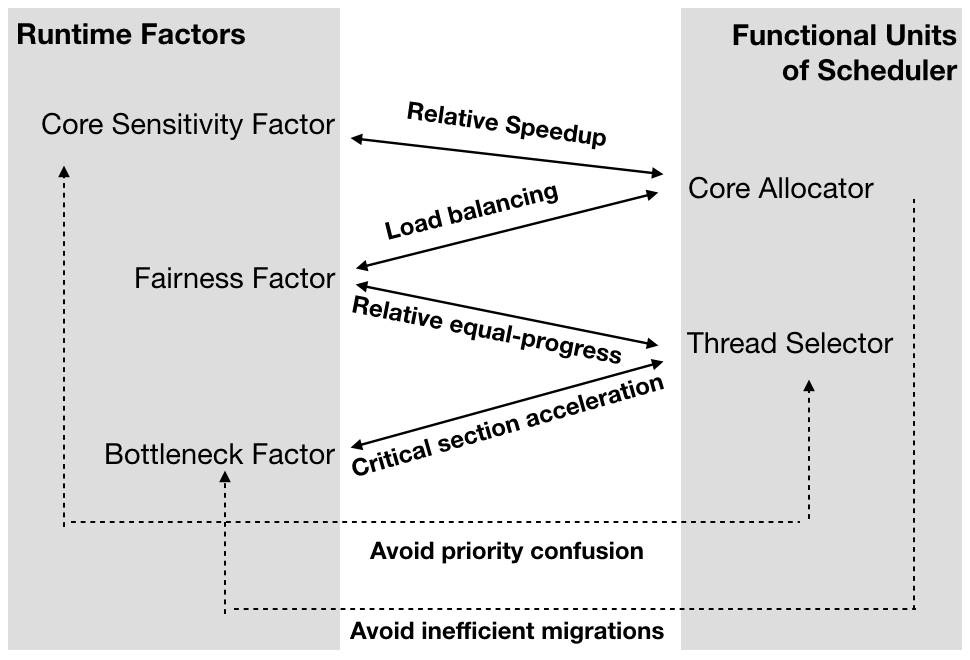
\includegraphics[scale=0.4]{figures/mfa.png}
\caption{Analytical model of runtime factors and relationships with functional units in Scheduler}
\label{figure:f1}
\end{figure} 

\subsection{Runtime Factors Analysis}
The overall analytical model of runtime factors and functional units in scheduler is shown in Fig. \ref{figure:f1}. We describe it by analyzing each factor. 

\textbf{\textit{Fairness:}} The fairness factor is critical for system performance. A good schedule achieving relative fairness on AMPs can efficiently share the heterogeneous hardware and avoid idle resource as much as possible. To achieve the expected relative equal-progress between threads and load-balancing between cores, the core allocator should hold the duty to map ready threads relative uniformly, which can avoid frequent migrations by potential empty runqueue. The preemption triggering mechanism of thread selector is also related with the fairness factor as it determines the slice of a task running each time - a thread currently running on big cores should have relatively shorter time slice against its running on little cores to result in similar progress.
%The preemption should be triggered and the thread selector should be invoked less frequent on little cores than on big cores     

\textbf{\textit{Core Sensitivity:}} The core sensitivity issue should be mainly addressed by the core allocator and avoid to confuse the decisions of thread selector. For instance, a thread with higher predicted speedup should have more opportunities to be allocated and executed on a high-performance big core against a low speedup thread. But higher speedup and more sensitive on big core does not indicate any {\it emergency} to execute this threads amount all other ready threads during the runtime. No priority should be given to high-speedup threads for a thread selector, only if in a special case when a big core finishes its current task with an empty runqueue and all other big cores hold empty runqueue as well - so it needs to globally select a ready thread from a runqueue of little core and then relative higher speedup threads are better candidates. This special case won't even appear in large-scale parallel workloads scenarios where the number of co-executing programs is at least greater than the number of cores - there will always be waiting threads in a big core's runqueue based on fairness core allocation as no data-dependence between threads from different programs. 

\textbf{\textit{Bottleneck Acceleration:}} Threads from multi-thread program hold contended locks and thus block other parallel threads should be identified as bottleneck and be executed as soon as possible. In large-scale workloads scenarios where multiple multi-thread programs are co-executing on limited AMPs resources and multiple blocking threads waiting to be executed, the thread selector should take the main duty to select those bottlenecks and run the corresponding critical code segments in an efficient way without confused by the priority from core sensitivity. In detail, the thread selector triggered by big cores should always give higher priorities for a thread with higher blocking level against another thread with higher speedup level and lower bottleneck. It may preempt the running threads on little cores to accelerate them when suited. The thread selector triggered by little cores should also intend to select relative high blocking threads and accelerate them locally first, instead of trivially migrating it to big cores and waiting to be actual accelerated. 

\begin{figure}
\centering
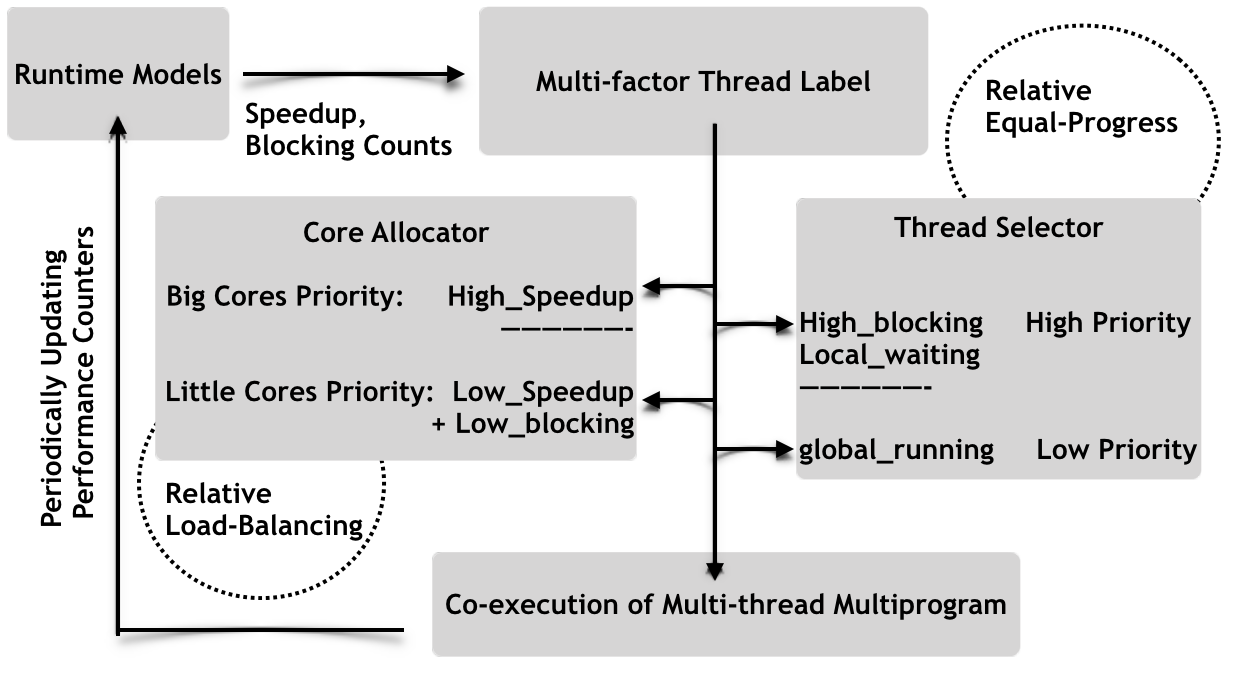
\includegraphics[scale=0.4]{figures/mfm.png}
\caption{Decentralized Model by Multi-factor collaboration and Distribution}
\label{figure:f2}
\end{figure} 

\subsection{Multiple Factors Distribution and Functional Units Collaboration}
Followed by the analysis on runtime factors, we can design a decentralized multi-factor model to address different issues by different functional units instead of a mixed multi-factor evaluator \cite{jibaja2016portable}.
%While the way we define whether a thread's relative speedup value is high or low is similar as in WASH based on hardware configuration - if we have same number of big and little cores, then we rank all ready threads based on its relative speedup and view the first half as high speedup value. 
The flowchart of our model is shown in Fig. \ref{figure:f2}. 

The multi-factor collaboration is achieved by a periodical multi-factor threads labeling progress. It labels the ready threads based on the runtime analysis from individual runtime models including speedup prediction and bottleneck identifier. Note that the metrics of whether a given thread is high speedup and blocking is not only based on the relative ranking between threads, but also having boundary conditions targeting hardware resource and experimental environments. For instance, no thread should be labeled as relative high-blocking during the initial time periods of experiments. We also setup an empirical lower boundary for threads with both very low speedup and blocking. It is mainly benefit in a mixed workloads scenario where we co-execute single and multi-thread multiprogram - a non-computing-intensive code segment from a single thread program can neither enjoy good performance gain on big cores nor block others. So we should better keep it in a little core and let other blocking threads to be executed before it. 

After the multi-level labeling process, multiple factors can be distributed to be concerned by either the core allocator or the thread selector or both of them together. Based on this decentralized model, the core allocator and thread selector handle different priorities queues from the set of ready threads - their decisions are not greedy on a mixed multi-factor ranking, but provide convenience for each others. 


\section{Runtime Design and Implementation}
We implement our approach on GEM5 simulator \cite{binkert2011gem5} by updating source code and constructing interfaces from the default Linux kernel v3.16 with CFS scheduler.

\subsection{Runtime Factors Implementations}
To implement the runtime multi-factor model, we update the main scheduler function \texttt{\_\_sched\_\_schedule()} of the Linux kernel by adding a thread labeling process as described in section 3.2 above. The similar method is applied when we re-implement the WASH scheduler by updating thread affinities without the help of VM. 

We present our implementation of each individual runtime factor below:

\textbf{\textit{Machine Learning based Speedup Prediction:}} Predicting relative speedup of each thread on heterogeneous cores is a main functional unit for any core sensitivity aware scheduler targeting AMPs. Our implementation of the speedup model follows a common approach in the literature \cite{van2013fairness,jibaja2016portable,saez2012leveraging}- an off-line trained predictive model applying on on-line. 

To construct the training set, we run all applications in single-program mode with two basic SMP configurations - full little cores and full big cores. We compute the speedup of each application between the heterogeneous cores and record all 225 performance counters from the simulated ARM cores in detailed CPU model from GEM5 \cite{binkert2011gem5} in full big core execution. Principal Component Analysis (PCA) is then applied to figure out several most relative and impotent counters. Finally, linear regression is applied on the applications set with selected counters and actual speedup to train the weight value of each counter. The selected counters and predictive linear speedup model targeting ARM big.LITTLE processors running on GEM5 are shown in table \ref{pca_sp}.  

\begin{table*}
  \caption{PCA Results and Speedup Model}
  \center
  \label{pca_sp}
   \scalebox{0.9}{
   \begin{tabular}{p{2cm} | p{6cm} | p {9cm} c c c}
 % \begin{tabular}{l c c c c}
   \toprule[1pt]
    \multicolumn{3}{c}{Selected GEM5 performance counters by PCA}\\
    \toprule[1pt]
     Index&  Name& Description \cite{binkert2011gem5} \\
     \midrule
     A: & fp\_regfile\_writes & number of integer regfile writes\\
     B: & fetch.Branches & number of branches that fetch encountered\\
     C: & rename.SQFullEvents & number of times rename has blocked due to SQ full\\
     D: & quiesceCycles & number of cycles  quiesced or waiting for an interrupt\\
     E: & dcache.tags.tagsinuse & cycle average of tags of dcache in use\\
     F: & fetch.IcacheWaitRetryStallCycles & number of stall cycles due to full MSHR\\
     G: & commit.committedInsts & number of instructions committed\\
     \midrule
     \toprule[1pt]
     \multicolumn{3}{c}{Linear predictive speedup model}\\
     \toprule[1pt]
     \multicolumn{3}{c}{2.6109+((0.0018*-0.185A)+(0.0259*0.187B)+(0.1047*0.194C)+(-0.023*0.238D)+(0.0492*-0.299E)+(-0.1388*-0.227F))/G}\\
    \bottomrule
  \end{tabular}}
\end{table*}



\textbf{\textit{Bottleneck Identification:}}
On modern Linux systems synchronization primitives are almost always implemented using kernel futexes, regardless of the threading library used. Futex-based mechanisms use a single atomic instruction in user space to acquire or release the futex, if it is uncontested. Otherwise, it triggers a system call which forces the thread to sleep or wakes up sleeping threads, respectively.

This gives us a convenient single point where we can monitor blocking patterns between threads. We first add code in \texttt{futex\_wait\_queue\_me()} and \texttt{futex\_lock\_pi()}, right before the active thread starts waiting on a futex. We record the current time and store it in the \texttt{task\_struct} of the thread. We then insert code in \texttt{wake\_futex()} and \texttt{wake\_futex\_pi()}, right before the waiting task is woken up by the thread releasing the futex. There we calculate the length of the waiting period and we accumulate it in the \texttt{task\_struct} of the thread releasing the futex. This way we are able to measure the cumulative time each thread has caused other threads to wait. We use this as our metric of thread criticality for the rest of the paper.

\textbf{\textit {Speedup based Scale-slice Preemption:}} Although we implement our scheduler on Linux kernel by fully re-writing both the core allocator and thread selector, the underlining preemption mechanism of Linux is applying the visual runtime {\it vruntime} in CFS with red-black tree data structure - whenever a new task is enqueued, a preemption wake-up function is invoked to check whether the new coming task should preempt the current task by computing the difference in vruntime and comparing with a boundary. 

To achieve relative equal-progress on AMPs, threads running on different types of cores should have relative different time slice instead of completely fairness on time. We update the default preemption wake-up function \texttt{wakeup\_preempt \_entity()} in Linux by constructing an interface to the GEM5 simulator. We apply our runtime speedup model to update the vruntime of current task by overing it with the thread's speedup value if the triggering core is a big core. 




\subsection{Scheduling Algorithm Design and Implementation}
\begin{algorithm}
\caption{Collaborated AMPs Scheduler with Runtime Factors Support}
\label{alg:1}
\begin{algorithmic}[1]
\STATE core\_alloctor\_(thread\_struct\ $t$)\{
%\FOR {$t : ready\_threads$}
%\IF {t->high\_speedup() \& t->high\_block()}
\IF {t->high\_speedup}
\RETURN rr\_allocator\_(big\_cores)
\ENDIF
\IF {t->low\_speedup \& t->low\_block \& !unique(t->tgid)}
\RETURN rr\_allocator\_(little\_cores)
\ENDIF
\RETURN rr\_allocator\_(cores)
\STATE \}
\STATE thread\_selector\_(core\_struct\ $c$)\{
%\IF {c->cur \& !(preempt_wakeup)}
\IF {!empty(c->rq)}
\RETURN max\_block\_(c->rq)
\ENDIF
%\IF {c->type == big}
\IF {!empty(c->sched\_domain->rq)}
\RETURN max\_block\_(c->sched\_domain->rq)
\ENDIF
\IF {c->cpu\_mask == big}
%\FOR {t : little\_core->cur}
%\STATE candidates.enqueue(t)
%\IF {!empty(candidates)}
\RETURN  max\_block\_(c->sched\_domain\_little->cur)
\ENDIF
%\ENDFOR
%\ENDIF
%\FOR {t : other\_little\_core->rq}
%\STATE candidates.enqueue(sorted\_speedup(t))
%\ENDFOR
%\IF {!empty(candidates)}
%\RETURN  max\_block\_(candidates)
%\ENDIF
%\ENDIF
%\FOR {t : other\_core->rq}
%\STATE candidates.enqueue(reversed\_speedup(t))
%\ENDFOR
\RETURN idle
\STATE \}
\end{algorithmic}
\end{algorithm}

Our scheduling algorithm is implemented by fully overriding the default task selector \texttt{pick\_next\_task\_fair()} and core allocator \texttt{select\_task\_rq\_fair()} in Linux kernel supported by the runtime factors. The pseudo-code of our scheduling algorithm is shown in Alg. \ref{alg:1}. 
Applied from common Linux notations, we use $rq$ to represent runqueue and $cur$ to represent the current task of a core in our code. We describe its two main functions below:

\textbf{\textit{Hierarchical Core Allocator:}}
When a thread is ready to be executed, whether it is just forked or waked up, the core allocator will be invoked to allocate this thread to a possible core's runqueue. To achieve relative load balancing and consider the influence from core sensitivity factor, we involve a hierarchical round-robin mechanism \texttt{rr\_allocator\_()}. Indicated by the speedup and blocking labels, threads are allocated to different core groups. Threads with high speedup level will be round-robin allocated in big core clusters (line 3). Low speedup and low blocking thread will only round-robin in little core clusters (line 5). A technical issue here is we need to distinguish threads from single-thread programs - those threads will definitely not block others and may not have a high speedup but we should not bind them to little cores. They can be easily detected by the allocator by checking whether there are ready threads whose group pid (t->tgid) equals to any others (line 5). To fill the gap of different core clusters, remain ready threads (usually with normal speedup level and tiny block) will be relatively equal allocated to both core types by \texttt{rr\_allocator\_(core)} - this final round-robin shares counters with the first two big/little core specific round-robin to achieve overall load balancing (line 6).  

\textbf{\textit{Bias-global Thread Selector:}}
The thread selector is based on the principle of accelerating the most critical/blocking thread as soon as possible shown in line 10, 12, 14. Triggered by different cores, the selector always try to return  a local candidate first instead of invoking additional migrations (line 10). When there is no local waiting thread and migration is useful, cores give priority for candidate thread waiting on others' runqueue and then highest blocking thread will be selected.
To reduce the overhead of accessing global CPUs states, we follow the same principle of the default Linux CFS scheduling domain (\texttt{struct sched\_domain}) - returning the best candidate thread from the local core group first (line 12).
Further, we allow a big core to select and preempt a running thread on little core to accelerate it (line 13,14). Idle resource will only happen when there is no any possible and useful work to be done (line 15) - For instance, we do not allow a little core to preempt a big core's execution. 

In summary, the thread selector still do as a global scheme that each core can select threads from all others' runqueue when needed but bias on the bottleneck and core sensitivity factors. 
Note that the relative equal-progress for achieving fairness is addressed by the scale-slice preemption checker instead of the thread selector - we give thread relative slice by avoiding triggering useless thread selections.

\textbf{\textit{Discussion:}}
This section provides a case study of implementing our scheduling framework targeting simulated ARM architectures and processors on GEM5.  However, the underlining general procedure and model can be easily implemented on real processors by using their hardware performance monitor events (PMU). For instance, we can input 150 PMU events \cite{ARMA57} of ARM Cortex-A57/A53 to the PCA process to build up corresponding speedup model when implement on real ARM cores.
%To further minimize the overhead of accessing global CPUs states to implement our approach on real systems, the thread selector can be configured to check other cpus one by one instead of 


\section{Experimental Evaluation}
 \begin{table*}
  \caption{Workloads Compositions}
  \center
  \label{WC}
   \scalebox{0.9}{
   \begin{tabular}{p{1.5cm} |p{5.5cm} || p{1.5cm} |p{9cm} }
     \toprule[1pt]
     \multicolumn{4}{c}{Multi-thread Multiprogram Workloads from PARSEC3.0 and SPLASH-2}\\
     \toprule[1pt] 
    2B-1 &blackshcoles - radix &4B-1 &blackshcoles - bodytrack - radix - lu\_ncb\\
    2B-2 &fft - swaptions &4B-2 &fft - radix - blackscholes - fluidanimate\\
    2B-3 &lu\_cb - dedup  &4B-3 &lu\_cb - fft - dedup - fluidanimate\\
    2B-4 &lu\_ncb - bodytrack &4B-4 &lu\_cb - lu\_ncb - bodytrack - dedup\\
    2B-5 &ferret - fluidanimate &4B-5 &radix - lu\_ncb - lu\_cb - fft\\
    2B-6 &radix - lu\_ncb &4B-6 &blackscholes - bodytrack - dedup - fluidanimate\\
    2B-7 &ocean\_cp - fft &4B-7 &radix - ocean\_cp - blackscholes - swaptions\\
    2B-8 &blackscholes - bodytrack &4B-8 &lu\_ncb - fft - ferret - freqmine\\
    2B-9 &dedup - fluidanimate &4B-9 &lu\_ncb - radix - ferret - swaptions\\
    2B-10 &lu\_cb - swaptions &4B-10 &ocean\_cp - fft - fluidanimate - swaptions\\
  %  6B-M &blackshcoles,bodytrack,dedup,radix,lu\_ncb,lu\_cb\\
  %  8B-M &blackshcoles,bodytrack,dedup,fluidanmiate,radix,lu\_ncb,lu\_cb,radiosity\\
  %  12B-M &blackshcoles,bodytrack,dedup,fluidanmiate,streamcluster,swaptions,radix,lu\_ncb,lu\_cb,radiosity,ocean\_cp,fft\\    
     \midrule
     \toprule[1pt]
     \multicolumn{4}{c}{Multi/Single-thread Multiprogram Workloads from PARSEC3.0, SPLASH-2 and SPEC2006}\\
     \toprule[1pt]  
    3B-1 &blackshcoles - radix - mcf &6B-1 &blackshcoles - bodytrack - radix - lu\_ncb - mcf - bzip2\\
    3B-2 &fft - swaptions - mcf &6B-2 &fft - radix - blackscholes - fluidanimate - mcf - bzip2\\
    3B-3 &freqmine - swaptions - mcf &6B-3 &blackscholes - dedup - freqmine - swaptions - mcf - bzip2\\
    3B-4 &blackscholes - freqmine - bzip2 &6B-4 &lu\_cb - lu\_ncb - bodytrack - dedup - mcf - bzip2\\
    %3B-5 &ocean\_cp - fluidanimate - mcf &6B-5 &radix - lu\_ncb - lu\_cb - fft - mcf - bzip2\\
    3B-5 &radix - lu\_ncb - bzip2 &6B-5 &radix - lu\_ncb - lu\_cb - fft - mcf - bzip2\\
    3B-6 &fluidanimate - freqmine - bzip2 &6B-6 &blackscholes - freqmine - swaptions - fluidanimate - mcf - bzip2\\
    3B-7 &blackscholes - fluidanimate - bzip2 &6B-7 &lu\_ncb - ocean\_cp - bodytrack - swaptions - mcf - bzip2\\
    3B-8 &dedup - fluidanimate - bzip2 &6B-8 &lu\_cb - ocean\_cp - dedup - swaptions - mcf - bzip2\\
    3B-9 &lu\_cb - swaptions - bzip2 &6B-9 &ocean\_cp - fft - fluidanimate - swaptions - mcf - bzip2\\
 %   7B-MS   &blackshcoles,bodytrack,dedup,radix,lu\_ncb,lu\_cb,mcf\\
 %   11B-MS &blackshcoles,bodytrack,dedup,canneal,swaptions,radix,lu\_ncb,lu\_cb,radiosity, bzip2,mcf\\ 
  %  15B-MS &blackshcoles,bodytrack,dedup,fluidanmiate,streamcluster,canneal,swaptions,radix,lu\_ncb,lu\_cb,radiosity, ocean\_cp,fft,bzip2,mcf\\   
  % &6B-7 &radix - ocean\_cp - blackscholes - swaptions - mcf - bzip2\\
    \bottomrule
  \end{tabular}}
\end{table*}
\subsection{Experimental Setup}
\textbf{\textit{Experimental Environment and Hardware Setup:}} The experiments are running on GEM5 simulator configured by ARM big.LITTLE architectures with multiple out-of-order 2GHz CortexA57 big cores and multiple in-order 1.2GHz CortexA53 little cores. We test on 2-big-2-little and 4-big-4-little configurations, separately. Each core associated L1 data cache, L1 instruction cache and L2 cache connected with NoC. There is no cache interference based on this architecture as described in \cite{kim2018exploring}.

\textbf{\textit{Workloads:}} The workloads we evaluated are multi-thread applications ({\it blackscholes, bodytrack, dedup, swaptions, freqmine, ferret and fluidanmiate}) mainly from PARSEC3.0 \cite{bienia11benchmarking}. It is a common issue that GEM5 simulator does not support all PARSEC3.0 benchmarks well \cite{endo2014micro}, so we also applied several more SPLASH2 benchmarks \cite{woo1995splash}: {\it radix, lu\_ncb, lu\_cb, ocean\_cp and fft}. We also considered two more single-thread benchmarks ({\it mcf, bzip2}) from SPEC2006 \cite{henning2006spec} to make the tested multiprogram workloads further complicated. 
%and () from SPLASH2 \cite{woo1995splash} benchmark suits and single-thread applications ({\it mcf, bzip2}) from SPEC2006. 
We mix those benchmarks to construct different workloads with either multiple multi-thread applications or mixed multiple multi-thread and single-thread applications. We do not test our approach on multiple sing-thread workloads scenarios as they are not the targeting scopes of our approach and efficient mix-critical model \cite{han2018multicore} has been exhibited for those scenarios. 

The number of parallel threads for benchmarks from SPLASH2 can be setup easily as in input arguments, while for PARSEC benchmarks, we only setup the lower bound of threads and the program will then determines the actual number of threads based on the relationships described in \cite{southern2016analysis}. To avoid dominating system performance by a single benchmark in each workload, we normalized the number of threads from different benchmarks to be similar and keep the input sizes of all applications to be {\it simsmall}. 
%The only exception is on benchmark {\it streamcluster} from PARSEC3.0 - it is a known issue \cite{southern2016analysis,roth2012deconstructing} that increasing the number of threads to be greater than 4 will significantly decrease the performance of this benchmark because of its barrier based synchronization.

Mixed from the original benchmarks, we generate multiple {\it 2-benchmarks, 3-benchmarks, 4-benchmarks and 6-benchmarks} multiprogram workloads for the evaluation and their compositions are listed in table \ref{WC}. For easy illustration, we use $\alpha$B-$\beta$ to name a workload, where $\alpha$B is the number of benchmark it contains and $\beta$ is the index of this workload.



\textbf{\textit{Metrics:}} The system metrics for multiple multi-thread workloads evaluation we considered are updated {\it Average Normalized Turnaround Time} (ANTT) and {\it System Throughput} (STP). As verified in \cite{eyerman2008system}, ANTT and STP are efficient system performance metrics for multiprogram co-execution on multicore processors. 

Their original definitions were based on SMPs, so the baseline performance of each application is obtained by running it in single-program mode by all multicore resources. While in AMPs environment, the heterogeneity from different cores will influence the performance of scheduler. To avoid this problem and obtain a suited baseline, we update the hardware configuration to be full of big cores when running single-program mode. We denote the total turnaround time of each multi-thread application $i$ under multi-program mode with AMPs and single-program mode with corresponding full-big SMPs as $T^{M}_i$ and $T^{SB}_i$, respectively.

Thus, we extend definitions of ANTT and STP across $n$ co-executing applications in multiprogram workloads on AMPs to be {\it Heterogeneous Average Normalized Turnaround Time} (H\_ANTT) and {\it Heterogeneous System Throughput} (H\_STP) as following:
$$ H\_ANTT = \frac{1}{n}\sum^{n}_{i=1}\frac{T^{M}_i}{T^{SB}_i}$$
$$ H\_STP = \sum^{n}_{i=1}\frac{T^{SB}_i}{T^{M}_i}$$

Similar with definitions of ANTT and STP, H\_ANTT is lower the better while H\_STP is higher the better. To better present our experimental results against the default Linux scheduler, we further  normalize results from each approach by dividing the original value against the results of Linux CFS on the same hardware configuration.

In multi-thread single-program workloads, we use the {\it Heterogeneous Normalized Turnaround Time} (H\_NTT) to present the results:
$$ H\_NTT = \frac{T^{M}}{T^{SB}}$$
It represents how much turnaround time slowdown of the tested workload on AMPs ($T^{M}$) against corresponding full-big core SMPs execution ($T^{SB}$) - lower the better. We do not consider system throughput for single-program executions.


\textbf{\textit{Comparisons:}}
Based on the demonstration and analysis in the background section above, we compare against both an re-implemented version of the stats-of-the-art WASH scheduler and the default Linux CFS scheduler. Our re-implemented version of WASH does exactly same as the original version by updating the thread affinity periodically based on the WASH algorithm and then leaves the final thread selection to the CFS. The only difference is we obtain performance counters from GEM5 simulator and change the thread affinities by updating the Linux kernel directly instead of applying the Java VM. 

\begin{figure}
\centering
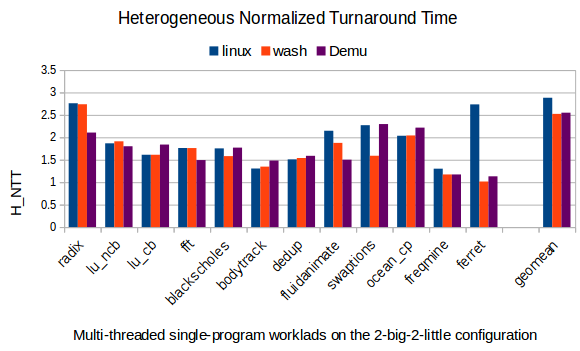
\includegraphics[scale=0.4]{figures/MSW.png}
\caption{Heterogeneous Normalized Turnaround Time (H\_NTT) of Multi-thread Single-program Workloads from PARSEC3.0 and SPLASH-2.}
\label{MSW}
\end{figure}  
\begin{figure*}
\centering
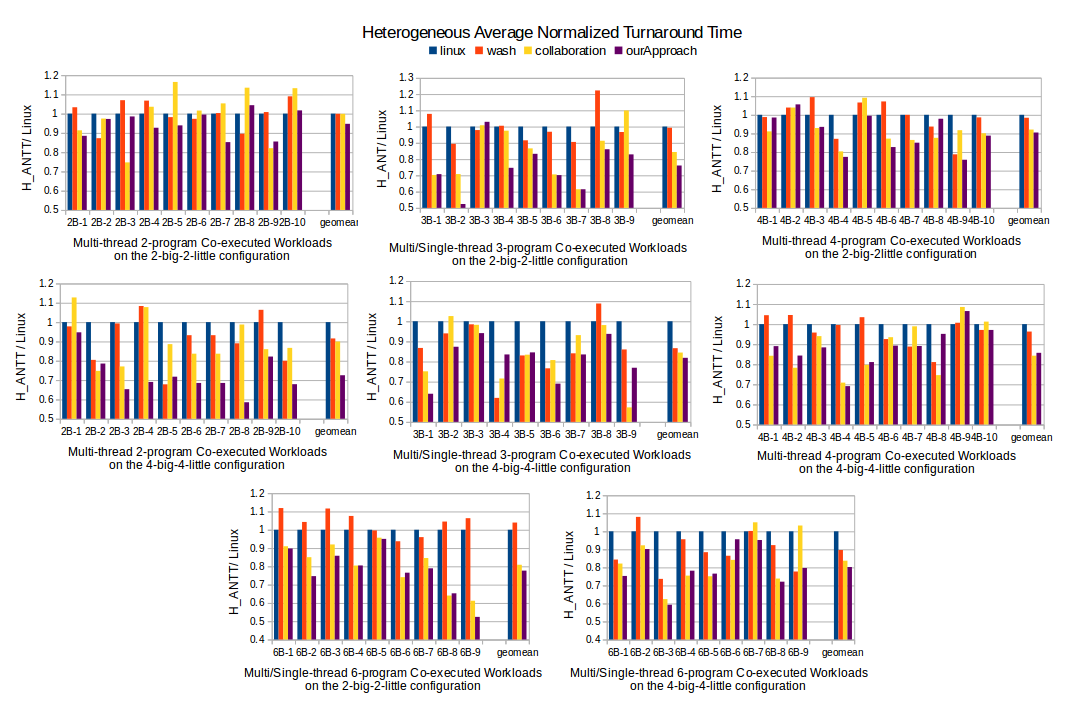
\includegraphics[scale=0.5]{figures/HANTT.png}
%{figures/M24W.png}
\caption{Heterogeneous Average Normalized Turnaround Time (H\_ANTT)  of Multi-thread Multiprogram Co-executed Workloads from PARSEC3.0, SPLASH-2 and SPEC2006 on 2-big-2-little and 4-big-4-little configurations.}
\label{M24W}
\end{figure*}

\subsection{Experimental Results and Analysis}



\subsubsection{Multi-thread Single-program Workloads}
Multi-thread single-program scheduling is the mainly targeting case for most of the research on AMP-aware schedulers. As discussed in the background section, WASH is the state-of-the-art approach which we re-implemented and compared against here with the default Linux CFS and our approach. We run 12 multi-thread benchmarks individually on a 2-big-2-little configuration and report their H\_NTT as shown in figure \ref{MSW}.

The performance of single multi-thread application execution is heavily influenced by the application. Both our approach and the WASH heterogeneous-aware scheduler can achieve up-to 60\% performance gain against Linux CFS on the {\it ferret} benchmark - its pipelined parallel model leads to a significant asymmetry between multiple threads, which is easy to be detected by runtime and then accelerated. 
%Our approach can achieve up-to 20\% performance gain on certain workloads ({\it radix, fluidanimate}) while also at most 20\% worse than WASH in the worst case ({\it swaptions}). 
Although Linux CFS is totally unaware of AMPs and simply keeps completely fairness, the more frequent migrations and the not 100\% precise off-line trained speedup model used by our approach and WASH may also results in a slightly worse solution than Linux sometime on certain workloads scenarios ($\it bodytrack, dedup$) - similar issues common happened in other state-of-the-art work \cite{jibaja2016portable} and appeared in our multiprogram experiments later as well.

As for the geomean of the multiple tests, both our approach and WASH results in around 5\% performance gain against Linux. WASH only results in around 0.5\% performance gain than us in this case, so we claim that our approach do not make trouble and still compatible with the state-of-the-art even in its mainly targeting case. 

Although our approach is not principally designed for single-program workloads, the experimental results have demonstrated a significant advantage of our decentralized multi-factor model on multi-thread benchmark with always-on lock-based synchronizations  ($fluidanimate$). As described in \cite{bienia08characterization}, $fluidanimate$ has around 100x more lock-based synchronizations than other PARSEC benchmarks, our collaborated core allocation and thread selection policy can accelerate those bottlenecks efficiently and locally during runtime.  



\subsubsection{Multi-thread Multi-program Workloads}
Multi-thread multi-program scheduling is the mainly target of our approach. We tests on multiple 2-program, 3-program, 4-program and 6-program workloads with different benchmark combinations on both 2-big-2-little and 4-big-4-little configurations. 

We also implement a collaboration-only approach for further comparison in those workload cases. This approach applies the same multi-factor mixed classifier from WASH instead of our multi-factor decentralized model - it achieves the basic collaboration between core allocator and thread selector by under the same guideline from the classifier instead of only updating the thread affinities as WASH.

\begin{figure*}
\centering
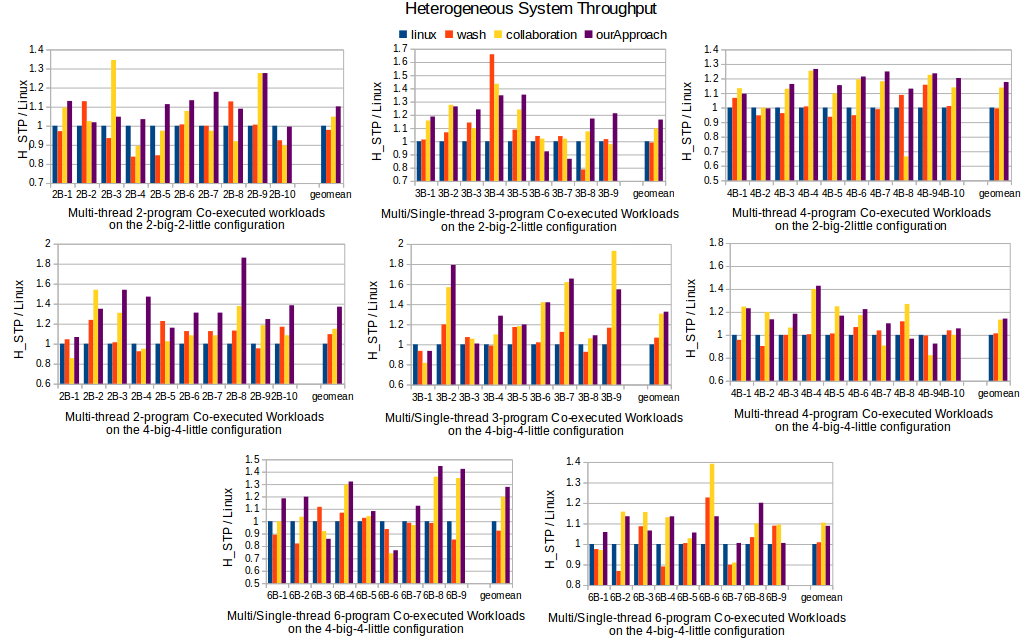
\includegraphics[scale=0.5]{figures/HSTP.png}
\caption{Heterogeneous System Throughput (H\_STP)  of Multi-thread Multiprogram Co-executed Workloads from PARSEC3.0, SPLASH-2 and SPEC2006 on 2-big-2-little and 4-big-4-little configurations..}
\label{M36W}
\end{figure*} 
\textbf{\textit{Heterogeneous Average Normalized Turnaround Time:}}
The results on Heterogeneous Average Normalized Turnaround Time (H\_ANTT) of the tested workloads are shown in the figure \ref{M24W}.  Results are come from either the 2-big-2-little configuration and 4-big-4-little results as indicated in the X-axis title of each graph. 

Instead of multi-thread single-program workloads, runtime communications and synchronizations are becoming more frequent during the co-execution of multi-thread multiprogram workloads - Multiple bottlenecks and high speedup threads waiting to be executed becomes an always-on scenario and our approach shows its truly advantage from those workloads.
%The results on 2-benchmark workloads are shown in the upper two graphs of figure \ref{M24W}.
For multiprogram co-executed workloads composed fully by multi-thread benchmarks, our approach can achieve around 8\%-10\% performance gain against both Linux CFS and WASH scheduler on either 2-program or 4-program workloads on the 2-big-2-little configuration as demonstrated by the geomean of results. The advantages from our approach are more significant and overall performance gain reaches to 15\%-26\% when test on 4-big-4-little configuration. The collaboration-only approach can also do better than both Linux and WASH, but not better than our final decentralized model based approach in most cases. 

Special cases of multi-thread multi-program workloads are workloads containing both single-thread and multi-thread benchmarks. Our proposed decentralized multi-factor model do significantly better on those workloads - A single-thread benchmark mixed in multi-thread benchmarks results in a non-block but sometime high speedup thread during runtime. Based on the relative equal-progress round-robin execution, our approach can always give relative lower priority of this {\it heavy non-bottleneck} thread to reduce the influence of it. Multi-factor mix-model may give higher priority of this thread than locking threads if it holds high speedup, which leads to a bad system performance. 
For those workloads composed by mixed of multi-thread and single-thread benchmarks, our approach can achieve up-to 20\% performance gain against both Linux CFS and WASH for most experimental scenarios.
%(6-program workloads on the 2-big-2-little configuration) while around 10\% performance gain in other cases. 
%Note that the collaboration-only approach without the technical hint on single-thread detection may either suffer a disaster or obtain a good fortune by binding single-thread program to little cores if it always get low speedup, which leads to very unstable performance of this approach - it can achieve up-to 40\% performance gain against Linux on a workload (3B-9 on the 4-big-4-little configuration) whilst suffer a more than 40\% slowdown (3B-4 on the 4-big-4-little configuration) against Linux as well and overall worse than all other approaches on certain  workload scenarios (3-program workloads on 4-big-4-little configuration).

While there may still be a few $symmetric$ workloads cases based on some certain benchmark combinations and hardware configurations, where threads are doing similar job with equally partitioned data - similar with findings from others previous research \cite{jibaja2016portable}, we find the default Linux CFS scheduler do slightly better in those cases as AMP-aware scheduler only adding some useless runtime overhead without a significant change of schedules. In conclusion, our proposed approach can do better than other approaches on more than 96\% test cases (73/76) and keep better on the geomean results for all workload scenarios.  
%our approach can achieve up-to 20\% performance gain of H\_ANTT on 4-program workloads against both Linux (4B-4,4B-8) and Wash (4B-6) and up-to 15 \% performance gain  


\textbf{\textit{Heterogeneous System Throughput:}}
The results on Heterogeneous System Throughput (H\_STP) of the tested workloads are shown in the figure \ref{M36W}.  Results are come from either the 2-big-2-little configuration and 4-big-4-little results as indicated in the X-axis title of each graph. 

Our proposed approach by accelerating multiple bottlenecks locally and simultaneously is more suited to avoid idle resource which leads to a more significant improvement on the system throughput against turnaround time. Based on the results from all 76 test cases, our approach can achieve better results than both Linux and the AMP-aware WASH scheduler for the geomean results on most of workload and configuration scenario. It can achieve up-to around 80\% performance gain for certain workload combinations (2B-8) for the 4-big-4-little configurations and up-to 40\% performance gain (6B-8,6B-9) for the 2-big-2-little configuration. 
%Towards all 76 individual cases, other approaches only better than us on 3 cases and our approach only less than 10\% worse than them in the worst case (3B-6 on the 2-big-2-little configuration). 
The collaboration-only approach can also do better than both Linux and WASH in most cases but worse than our final approach equipped with the multi-factor decentralized model.

%with up-to 34\% improvement of H\_STP against other approaches. It does at most 15\% worse than WASH in the worst case (2B-2). Linux can also do slightly better than both WASH and our approach for some workloads (2B-10). As for the geomean of the multiple tests, our approach results in around 5\% performance gain of H\_ANTT against Linux CFS, while both WASH and the collaboration-only approach can not do better than Linux. The collaboration-only approach can achieve around 5\% improvement of H\_STP against Linux and WASH, and the improvement grows up to more than 10\% by applying our final approach. 

%The results on 4-benchmark workloads are shown in the lower two graphs of figure \ref{M24W}.Our approach can achieve up-to 39\% performance gain of H\_ANTT on certain workloads (4B-7) and up-to 40\% improvement of H\_STP on (4B-7). It does at most 10\% worse than WASH in the worst case (4B-9). Linux can also do better than both WASH and our approach for some workloads (4B-9). As for the geomean of the multiple tests, both the collaboration-only and our final approach results in around 9\% performance gain of H\_ANTT against WASH and 7\% against Linux. The collaboration-only approach can achieve around 14\% improvement of H\_STP against Linux and WASH, and the improvement grows up to more than 19\% by applying our final approach.  

%\textbf{\textit{Multi/single-thread Multi-program Workloads}}
 
%The results on 3-benchmark workloads are shown in the upper two graphs of figure \ref{M36W}.
%Our approach can achieve up-to 54\% performance gain of H\_ANTT on certain workloads (3B-2) and up-to 33\% improvement of H\_STP on (3B-1). It can always keep better than WASH in the all workload cases. Linux can also do slightly better than both WASH and our approach for some workloads (3B-6). As for the geomean of the multiple tests, the collaboration-only approach obtains around 5\% performance gain of H\_ANTT against Linux and WASH is not better than Linux. Our final approach can achieve 20\% performance gain against Linux and 25\% against WASH. The collaboration-only approach can achieve around 13\% improvement of H\_STP against Linux and WASH, and the improvement grows up to more than 18\% by applying our final approach.  
 
%The results on 6-benchmark workloads are shown in the lower two graphs of figure \ref{M36W}.
%Our approach can achieve up-to 54\% performance gain of H\_ANTT on certain workloads (6B-3) and up-to 46\% improvement of H\_STP on (6B-4). Linux can also do slightly better than both WASH and our approach for some workloads (6B-1,6B-5). As for the geomean of the multiple tests, the collaboration-only approach obtains around 17\% performance gain of H\_ANTT against Linux and WASH is not better than Linux. Our final approach can achieve 23\% performance gain against Linux and 27\% against WASH. The collaboration-only approach can achieve around 16\% improvement of H\_STP against Linux and WASH, and the improvement grows up to more than 20\% by applying our final approach.  



\textbf{\textit{Experimental Summary}} As shown in the results, the state-of-the-art AMP-aware WASH scheduler targeting multi-thread single-program execution is generally not good for multi-thread multiprogram co-execution. The mixed priorities of threads from multi-factor model can not lead to a general better performance even against Linux. 

By achieving core allocator and thread selector collaboration to guarantee accelerating multiple high priority threads on multiprogram workloads, the scheduler begins to do better and show the truly advantage from AMPs. While this collaboration is still not efficient enough to handle the always-on bottlenecks appears in multiprogram workloads. By equipped with the multi-factor decentralized model, our final approach can efficiently partition and address runtime issues - keep high-speedup threads on big cores whilst accelerate multiple bottlenecks locally and simultaneously. This results in a significantly better results than both the AMP-aware WASH scheduler and Linux CFS for multi-thread multiprogram co-execution on AMPs.  

\section{Conclusion}
This paper present a novel OS scheduling framework targeting multi-thread multiprogram co-execution workloads on asymmetric multicore processors. We design the first ever multi-factor decentralized model to address multiple critical runtime scheduling issues efficiently and simultaneously, including relative fairness, bottleneck acceleration and core sensitivity analysis. 

Compared with the default Linux CFS scheduler and the state-of-the-art AMP-aware WASH scheduler, it achieves up-to 30\% performance gain in heterogeneous average normalized turnaround time (H\_ANTT) and up-to 40\% increase on heterogeneous system throughput (H\_STP) in geomean targeting multi-thread multiprogram co-executed workloads. 
%It performs significantly better when workloads contain both multi-thread and single-thread applications achieving performance gain up to 54\% in average normalized turnaround time and 46\% increase on system throughput against both the previous approaches.

Our work aims to highlight the potential of further performance gain for AMP-aware scheduler targeting multi-thread multiprogram co-execution and encourage following research by applying decentralized multi-factor runtime frameworks with core allocator and thread scheduler collaboration. 

%% Acknowledgments
\begin{acks}                            %% acks environment is optional
                                        %% contents suppressed with 'anonymous'
  %% Commands \grantsponsor{<sponsorID>}{<name>}{<url>} and
  %% \grantnum[<url>]{<sponsorID>}{<number>} should be used to
  %% acknowledge financial support and will be used by metadata
  %% extraction tools.
  This material is based upon work supported by the
  \grantsponsor{GS100000001}{National Science
    Foundation}{http://dx.doi.org/10.13039/100000001} under Grant
  No.~\grantnum{GS100000001}{nnnnnnn} and Grant
  No.~\grantnum{GS100000001}{mmmmmmm}.  Any opinions, findings, and
  conclusions or recommendations expressed in this material are those
  of the author and do not necessarily reflect the views of the
  National Science Foundation.
\end{acks}


%% Bibliography
%\bibliography{bibfile}
\bibliographystyle{plain}
\bibliography{references}
\end{document}
%% Appendix
%\appendix
\section{Appendix}
\begin{figure*}
\centering
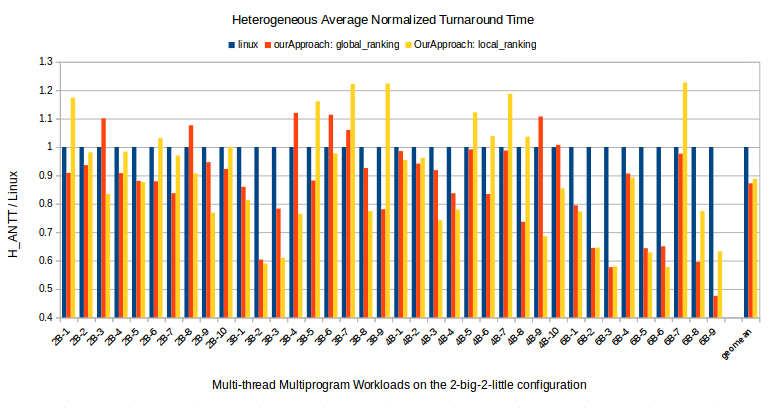
\includegraphics[scale=0.65]{figures/crank.png}
\caption{H\_ANTT Comparison between global ranking and local ranking  on Multi-thread Multiprogram Co-executed Workloads from PARSEC3.0, SPLASH-2 on the 2-big-2-little configuration}
\label{M36W}
\end{figure*}



%Text of appendix \ldots



\subsection{Bottleneck Identification and Acceleration}
Bottleneck can be defined as any code segment which threads contend. It is critical for performance of multicore systems on parallel executions: Like a barrier where multiple threads need to reach a synchronization point before others can make new progress. Other bottlenecks are such as critical sections of multi-thread programs and pipeline stages. Failure to accelerate bottleneck can lead to reduce or even stop speedup which could be expected from parallel executions on multicore processors. 

An efficient Bottleneck Identification and Scheduling (BIS) approach on AMPs was presented in \cite{joao2012bottleneck}. In addition of their previous efforts \cite{suleman2009accelerating} which can only accelerate one bottleneck at a time on single big core systems, BIS can identify which bottlenecks are most critical at any given time and accelerate them accordingly on big cores. The key idea is to measure the number of cycles spent by each thread when waiting for bottlenecks and then rank and accelerate those bottlenecks based on those values. It is mainly composed by twofolds:

\begin{itemize}
\item[1.] Bottleneck Identification: A bottleneck table (BA) is implemented in which each entry corresponds to a bottleneck and includes a thread waiting cycles field (WCT) to track this information. WCT value is computed by aggregating the number of threads who are waiting on this bottleneck. The critical bottlenecks are then identified by BA with $N$ highest WCT values where $N$ is based on the number of big cores in the system.
\item[2.] Bottleneck Acceleration: To decide whether a bottleneck should be accelerated by big cores, an acceleration index table (AIT) is created associated with each small core. The small cores send bottleneck execution requests based on the information from AIT and those requests are then enqueued in a scheduling buffer (SB) in big cores. SB is actually a priority queue which always run the oldest instance with highest WCT value. To avoid false serialisation and resource starvation, SB also implement an request abort function which will let the big core send back a bottleneck to small cores if this bottleneck does not have the highest WCT value and is ready to run on small cores.
\end{itemize}
Based on the core function from BIS, following approach has been developed in the same track, such as using a utility function to make more efficient bottleneck identification in \cite{joao2013utility} and designing mix-critical level to rank the threads more precisely in \cite{han2018multicore}. 


\subsection{Fairness and Load balancing}
Fairness, or guaranteeing all threads make equal progress is another critical factor of scheduling on heterogeneous multicore processors, especially when targeting on multi-thread workloads with barrier-synchronisation and multi-program workloads with quality-of-service (QoS) constraints.

Two fairness-aware scheduling methods are presented in \cite{van2013fairness}. 
\begin{itemize}
\item[1.] The first one is called $equal$-$time$ scheduling. It trivially keeps each thread to run on each type of cores in same amount of time slices and implemented by Round-robin or random selection of a thread which currently on small core to schedule on big core next. But it cannot imply truly fairness if threads experience different slowdown or speedup from different cores. 
\item[2.] A more advantage approach to handle this fact in their paper is called $equal$-$progress$ scheduling which guarantee each thread reach the equal progress on heterogeneous cores.  The key challenge of this approach is to estimate a big-versus-small-core scaling factor for all threads and then it can be used to compute the slowdown between running on heterogeneous cores and big cores in isolation.  There are three methods provided to obtain this factor: (1) sampling-based method which compute this factor during a sample phase as the ratio between CPI on different cores and then apply on symbiosis phase; (2) history-based method which is similar with the sampling way but records historical CPI values and continuously adjust the ratio; (3) model-based method which use a performance impact estimation (PIE) \cite{van2012scheduling} analytical model to estimate this factor with hardware support.
\end{itemize}
They also mentioned a $guaranteed$-$fairness$ approach based on their scheduler when system throughput need to be concern. A threshold of fairness can be setup and the scheduler will defers to a throughput-optimisation policy after this threshold reached. Overall, fairness-aware scheduler achieve 14\% performance gain on homogeneous multi-thread workloads and 32\% performance gain on heterogeneous multi-thread workloads on average against other schedulers. 

Note that the well-known Linux scheduler is also fairness-oriented which is based on complete fairness scheduling (CFS) \cite{li2009efficient}. Focusing on fairness and designing more efficient fairness-oriented metric functions or market-based metrics is always a main trend in the research community, more work are presented during recent years such as Uniformity \cite{kim2018exploring} and ReBudget\cite{wang2016rebudget}.

\subsection{Heterogeneous Core Sensitivity}
WASH \cite{jibaja2016portable} is the most state-of-the-art scheduler which provides a novel AMP-aware runtime environment which use dynamically analysis to classify application, identify bottleneck and prioritises threads based on single-ISA. It is the first work who can optimise critical path, core sensitivity, priorities and load balancing simultaneously. 

Compared with their previous statical $yin$ and $yang$ based scheduler \cite{cao2012yin} which always bind threads based on static classification, WASH algorithm dynamically and periodically use runtime information about core sensitivity, thread sensitivity and workload to schedule threads. The scheduler starts with scheduling application threads on big cores and VM threads on small cores, and then dynamically classify (scalable or not), prioritise and migrate threads guided by the runtime information.

They implement two models to record and provide those information.
\begin{itemize}
\item[1.] One is named a dynamic bottleneck analysis. The core function is to accelerate threads which hold contended locks by computing an ratio between the time this tread waits for another thread to release a lock and the total execution time of it so far. To prioritise among those threads, it select the one who make others wait the longest to big cores.
\item[2.] The second is a core sensitive predictor. It uses linear regression and Principal Component Analysis to learn most significant performance counters with corresponding weight. The selected counters include such as INSTRCUTIONS\_RETIRED and  L1D\_ALL\_REF:ANY for Intel processors and RETIRED\_UOPS and CPU\_CLK\_UNHALTED for AMD cores. Those counters can then be used to compute the speedup if we schedule a thread on big cores than on small cores. In detail, it involves two relative ranking function. The $ExecRank$ is an adjusted priority which shows how much performance gain can be achieved if the thread is on big cores by accumulating on retired instructions. The $LockRank$ is to show the bottleneck level based on the amount of time other threads have been waiting for it. 
\end{itemize}
Overall, WASH report a up-to 20\% performance gain and 9\% energy save against prior work on heterogeneous multicore AMD cores in different configurations. 

\begin{table}
  \caption{PCA Results and Speedup Model}
  \center
  \label{pca_sp}
   \scalebox{0.9}{
   \begin{tabular}{p{1cm} p{3cm} | p {3cm} c c c}
 % \begin{tabular}{l c c c c}
   \toprule[1pt]
    \multicolumn{3}{c}{Selected GEM5 performance counters by PCA}\\
    \toprule[1pt]
     Index&  Name& Description \\
     \midrule
     A: & fp\_regfile\_writes & number of integer regfile writes\\
     B: & fetch.Branches & number of branches that fetch encountered\\
     C: & rename.SQFullEvents\\
     D: & quiesceCycles\\
     E: & dcache.tags.tagsinuse\\
     F: & fetch.IcacheWaitRetryStallCycles\\
     G: & commit.committedInsts\\
     \midrule
     \toprule[1pt]
     \multicolumn{3}{c}{Linear predictive speedup model}\\
     \toprule[1pt]
     \multicolumn{3}{c}{2.6109+((0.0018*-0.185A)+(0.0259*0.187B)+(0.1047*0.194C)}\\ 
     \multicolumn{3}{c}{+(-0.023*0.238D)+(0.0492*-0.299E)+(-0.1388*-0.227F))/G}\\
    \bottomrule
  \end{tabular}}
\end{table}